\documentclass{standalone}
\usepackage{tikz}
\usetikzlibrary{patterns, positioning}


\begin{document}
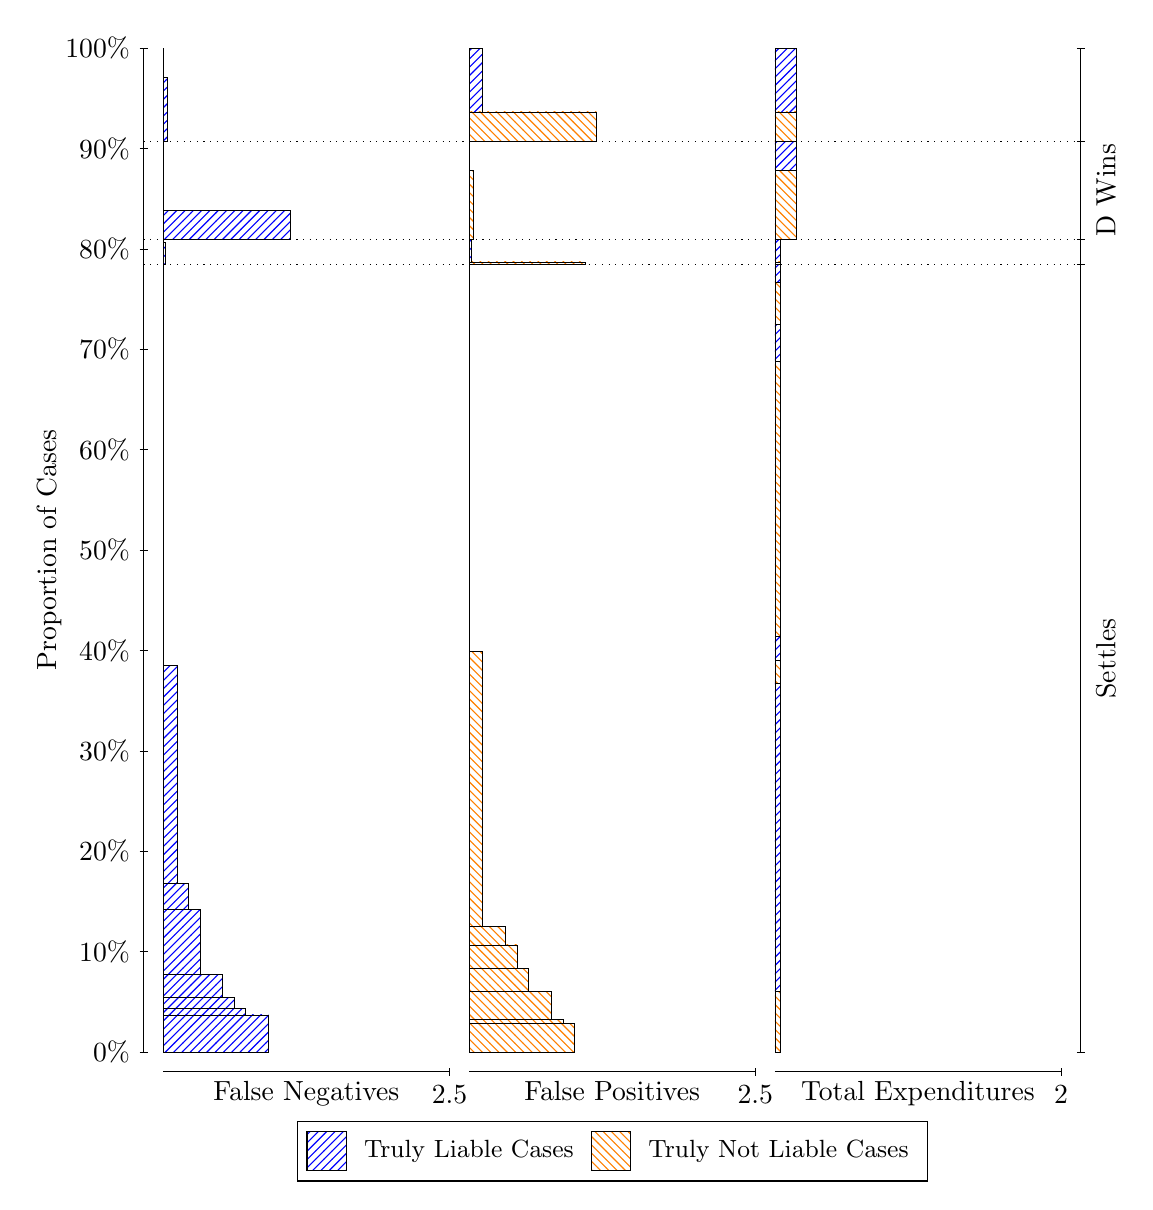
\begin{tikzpicture}
\draw[black, very thin] (1.5,1.75) -- (1.5,14.5);
\node[rotate=90, text=black, anchor=center] at (0.3, 8.125) {Proportion of Cases};
\draw[black, very thin] (1.45,1.75) -- (1.55,1.75);
\node[text=black, anchor=east] at (1.45, 1.75) {0\%};
\draw[black, very thin] (1.45,3.025) -- (1.55,3.025);
\node[text=black, anchor=east] at (1.45, 3.025) {10\%};
\draw[black, very thin] (1.45,4.3) -- (1.55,4.3);
\node[text=black, anchor=east] at (1.45, 4.3) {20\%};
\draw[black, very thin] (1.45,5.575) -- (1.55,5.575);
\node[text=black, anchor=east] at (1.45, 5.575) {30\%};
\draw[black, very thin] (1.45,6.85) -- (1.55,6.85);
\node[text=black, anchor=east] at (1.45, 6.85) {40\%};
\draw[black, very thin] (1.45,8.125) -- (1.55,8.125);
\node[text=black, anchor=east] at (1.45, 8.125) {50\%};
\draw[black, very thin] (1.45,9.4) -- (1.55,9.4);
\node[text=black, anchor=east] at (1.45, 9.4) {60\%};
\draw[black, very thin] (1.45,10.675) -- (1.55,10.675);
\node[text=black, anchor=east] at (1.45, 10.675) {70\%};
\draw[black, very thin] (1.45,11.95) -- (1.55,11.95);
\node[text=black, anchor=east] at (1.45, 11.95) {80\%};
\draw[black, very thin] (1.45,13.225) -- (1.55,13.225);
\node[text=black, anchor=east] at (1.45, 13.225) {90\%};
\draw[black, very thin] (1.45,14.5) -- (1.55,14.5);
\node[text=black, anchor=east] at (1.45, 14.5) {100\%};

\draw[black, very thin] (13.4,1.75) -- (13.4,14.5);
\draw[black, very thin] (13.35,1.75) -- (13.45,1.75);
\node[anchor=west] at (13.35, 1.75) {};
\draw[black, very thin] (13.35,11.748) -- (13.45,11.748);
\node[anchor=west] at (13.35, 11.748) {};
\draw[black, very thin] (13.35,12.068) -- (13.45,12.068);
\node[anchor=west] at (13.35, 12.068) {};
\draw[black, very thin] (13.35,13.318) -- (13.45,13.318);
\node[anchor=west] at (13.35, 13.318) {};
\draw[black, very thin] (13.35,14.5) -- (13.45,14.5);
\node[anchor=west] at (13.35, 14.5) {};

\draw[black, very thin, pattern color=blue, pattern=north east lines] (1.75,1.75) rectangle (3.0852,2.2209);
\draw[black, very thin, pattern color=blue, pattern=north east lines] (1.75,2.2209) rectangle (2.7946,2.3031);
\draw[black, very thin, pattern color=blue, pattern=north east lines] (1.75,2.3031) rectangle (2.6492,2.4407);
\draw[black, very thin, pattern color=blue, pattern=north east lines] (1.75,2.4407) rectangle (2.5039,2.7396);
\draw[black, very thin, pattern color=blue, pattern=north east lines] (1.75,2.7396) rectangle (2.2133,3.5632);
\draw[black, very thin, pattern color=blue, pattern=north east lines] (1.75,3.5632) rectangle (2.0679,3.8872);
\draw[black, very thin, pattern color=blue, pattern=north east lines] (1.75,3.8872) rectangle (1.9226,6.6566);
\draw[black, very thin, pattern color=orange, pattern=north west lines] (1.75,6.6566) rectangle (1.75,11.748);
\draw[black, very thin, pattern color=blue, pattern=north east lines] (1.75,11.748) rectangle (1.7773,12.034);
\draw[black, very thin, pattern color=orange, pattern=north west lines] (1.75,12.034) rectangle (1.75,12.068);
\draw[black, very thin, pattern color=blue, pattern=north east lines] (1.75,12.068) rectangle (3.3668,12.441);
\draw[black, very thin, pattern color=orange, pattern=north west lines] (1.75,12.441) rectangle (1.75,13.318);
\draw[black, very thin, pattern color=blue, pattern=north east lines] (1.75,13.318) rectangle (1.8045,14.128);
\draw[black, very thin, pattern color=orange, pattern=north west lines] (1.75,14.128) rectangle (1.75,14.5);
\draw[black, very thin, pattern color=orange, pattern=north west lines] (5.6333,1.75) rectangle (6.9686,2.1169);
\draw[black, very thin, pattern color=orange, pattern=north west lines] (5.6333,2.1169) rectangle (6.8233,2.162);
\draw[black, very thin, pattern color=orange, pattern=north west lines] (5.6333,2.162) rectangle (6.6779,2.5209);
\draw[black, very thin, pattern color=orange, pattern=north west lines] (5.6333,2.5209) rectangle (6.3873,2.808);
\draw[black, very thin, pattern color=orange, pattern=north west lines] (5.6333,2.808) rectangle (6.2419,3.1095);
\draw[black, very thin, pattern color=orange, pattern=north west lines] (5.6333,3.1095) rectangle (6.0966,3.3438);
\draw[black, very thin, pattern color=orange, pattern=north west lines] (5.6333,3.3438) rectangle (5.8059,6.8419);
\draw[black, very thin, pattern color=blue, pattern=north east lines] (5.6333,6.8419) rectangle (5.6333,11.748);
\draw[black, very thin, pattern color=orange, pattern=north west lines] (5.6333,11.748) rectangle (7.1139,11.783);
\draw[black, very thin, pattern color=blue, pattern=north east lines] (5.6333,11.783) rectangle (5.6606,12.068);
\draw[black, very thin, pattern color=orange, pattern=north west lines] (5.6333,12.068) rectangle (5.6878,12.945);
\draw[black, very thin, pattern color=blue, pattern=north east lines] (5.6333,12.945) rectangle (5.6333,13.318);
\draw[black, very thin, pattern color=orange, pattern=north west lines] (5.6333,13.318) rectangle (7.2502,13.69);
\draw[black, very thin, pattern color=blue, pattern=north east lines] (5.6333,13.69) rectangle (5.7968,14.5);
\draw[black, very thin, pattern color=orange, pattern=north west lines] (9.5167,1.75) rectangle (9.5848,2.5209);
\draw[black, very thin, pattern color=blue, pattern=north east lines] (9.5167,2.5209) rectangle (9.5848,6.4379);
\draw[black, very thin, pattern color=orange, pattern=north west lines] (9.5167,6.4379) rectangle (9.5848,6.725);
\draw[black, very thin, pattern color=blue, pattern=north east lines] (9.5167,6.725) rectangle (9.5848,7.0239);
\draw[black, very thin, pattern color=orange, pattern=north west lines] (9.5167,7.0239) rectangle (9.5848,10.522);
\draw[black, very thin, pattern color=blue, pattern=north east lines] (9.5167,10.522) rectangle (9.5848,10.993);
\draw[black, very thin, pattern color=orange, pattern=north west lines] (9.5167,10.993) rectangle (9.5848,11.529);
\draw[black, very thin, pattern color=blue, pattern=north east lines] (9.5167,11.529) rectangle (9.5848,11.748);
\draw[black, very thin, pattern color=orange, pattern=north west lines] (9.5167,11.748) rectangle (9.5848,11.783);
\draw[black, very thin, pattern color=blue, pattern=north east lines] (9.5167,11.783) rectangle (9.5848,12.068);
\draw[black, very thin, pattern color=orange, pattern=north west lines] (9.5167,12.068) rectangle (9.7892,12.945);
\draw[black, very thin, pattern color=blue, pattern=north east lines] (9.5167,12.945) rectangle (9.7892,13.318);
\draw[black, very thin, pattern color=orange, pattern=north west lines] (9.5167,13.318) rectangle (9.7892,13.69);
\draw[black, very thin, pattern color=blue, pattern=north east lines] (9.5167,13.69) rectangle (9.7892,14.5);
\draw[black, dotted] (1.5,11.748) -- (13.4,11.748);
\draw[black, dotted] (1.5,12.068) -- (13.4,12.068);
\draw[black, dotted] (1.5,13.318) -- (13.4,13.318);
\draw[black, very thin] (1.75,1.5) -- (5.3833,1.5);
\node[text=black, anchor=north] at (3.5667, 1.5) {False Negatives};
\draw[black, very thin] (5.3833,1.45) -- (5.3833,1.55);
\node[text=black, anchor=north] at (5.3833, 1.45) {2.5};

\draw[black, very thin] (5.6333,1.5) -- (9.2667,1.5);
\node[text=black, anchor=north] at (7.45, 1.5) {False Positives};
\draw[black, very thin] (9.2667,1.45) -- (9.2667,1.55);
\node[text=black, anchor=north] at (9.2667, 1.45) {2.5};

\draw[black, very thin] (9.5167,1.5) -- (13.15,1.5);
\node[text=black, anchor=north] at (11.333, 1.5) {Total Expenditures};
\draw[black, very thin] (13.15,1.45) -- (13.15,1.55);
\node[text=black, anchor=north] at (13.15, 1.45) {2};

\node[text=black, centered, rotate=90] at (13.72, 6.7492) {Settles};

\node[text=black, centered, rotate=90] at (13.72, 12.693) {D Wins};


\draw (7.449999999999999,1.5) node[draw=none] (baseCoordinate) {};
\begin{scope}[align=center]
        \matrix[scale=0.5, draw=black, below=0.5cm of baseCoordinate, nodes={draw}, column sep=0.1cm]{
            \node[rectangle, draw, minimum width=0.5cm, minimum height=0.5cm, pattern color=blue, pattern=north east lines] {}; &
            \node[draw=none, font=\small, text=black] (B) {Truly Liable Cases}; &
            \node[rectangle, draw, minimum width=0.5cm, minimum height=0.5cm, pattern color=orange, pattern=north west lines] {}; &
            \node[draw=none, font=\small, text=black] (B) {Truly Not Liable Cases}; \\
            };
\end{scope}

\end{tikzpicture}
\end{document}